\section{Experimental Details and Supporting Analyses}
\label{app:details}

\subsection{Implementation}

Hidden states are extracted with a single forward pass over
\texttt{[BOS]} $+$ context $+$ phrase, with \texttt{output\_hidden\_states}
enabled. The BOS token is required: the state of a phrase's first token at
position $0$ differs substantially from its state at position $1$ after a BOS,
and omitting it produces degenerate patchscope outputs.\footnote{This was the
source of a long-lived bug in an earlier version of this work, in which
patchscope outputs for well-known phrases were unrelated to the input.}
Positions are enumerated from the first phrase token to the second-to-last; the
BOS and the final phrase token are never cut points.

For the Patchscopes readout, the states for all probed layers are stacked into
one batch and decoded in a single \texttt{generate} call, so the layer sweep
costs one generation pass rather than one per layer. Decoding is greedy
throughout, for both readouts, with \texttt{max\_new\_tokens} $= i+3$.

\subsection{Patchscope prompt ablation}

The prompt \texttt{"Repeat this: X"} offers one slot for the injected state.
Because the target is several tokens long, a natural worry is that one slot is
too little room. We reran the isolated-phrase sweep with
\texttt{"Repeat this: X X X X X"}, injecting the same state into five slots.
It does not help, and at longer distances it hurts: $27.4\%$ versus $30.9\%$ at
$i=3$, $15.8\%$ versus $19.4\%$ at $i=4$, and $12.4\%$ versus $16.5\%$ at
$i=5$. We therefore use the single-slot prompt throughout. The failure mode at
long $i$ is not a shortage of output positions.

\subsection{Replication across models}

\begin{table}[t]
\centering\small
\begin{tabular}{llrrrr}
\toprule
& & \multicolumn{4}{c}{$i$} \\
\cmidrule(lr){3-6}
\textbf{Model} & \textbf{Readout} & 2 & 3 & 4 & 5 \\
\midrule
\multicolumn{6}{l}{\textit{Phrase in isolation}} \\
OLMo-2-7B & patchscopes & 57.8 & 30.9 & 19.4 & 16.5 \\
OLMo-3-7B & patchscopes & 40.4 & 20.1 & 11.8 & 9.9 \\
OLMo-2-7B & generation & 59.2 & 31.2 & 20.6 & 17.6 \\
Qwen2.5-14B & generation & 54.3 & 28.4 & 18.8 & 17.4 \\
\midrule
\multicolumn{6}{l}{\textit{Phrase in natural context}} \\
OLMo-2-7B & patchscopes & 79.6 & 64.1 & 51.6 & 46.4 \\
OLMo-3-7B & patchscopes & 71.4 & 52.8 & 38.9 & 32.9 \\
OLMo-2-7B & generation & 84.0 & 64.8 & 55.6 & 53.6 \\
Qwen2.5-14B & generation & 84.8 & 66.2 & 57.4 & 54.7 \\
\bottomrule
\end{tabular}
\caption{Recovery rate (\%) across models, on the same phrase strings and
contexts. Each model uses its own tokenizer, so $i$ counts model-specific tokens
and the cut points need not coincide across rows. Patchscopes rows are the union
over all 32 layers. Qwen2.5-14B, at
roughly twice the parameters of OLMo-2-7B, is slightly behind it in isolation
and slightly ahead of it in context.}
\label{tab:replication}
\end{table}


Table~\ref{tab:replication} repeats the central measurement on OLMo-3-7B
(both readouts share the OLMo-2 protocol; note that this tokenizer does not
prepend a BOS token) and on Qwen2.5-14B (generation readout only). The
qualitative picture is stable across all three: anticipation several tokens
ahead, a large context effect, and a monotone decline with $i$. The absolute
levels differ, and not in the direction model scale would predict --- OLMo-3-7B
is consistently below OLMo-2-7B, and Qwen2.5-14B, at roughly twice the
parameters, trails OLMo-2-7B in isolation and leads it by one to two points in
context.

\subsection{Depth of first recovery}

\begin{figure}[t]
\centering
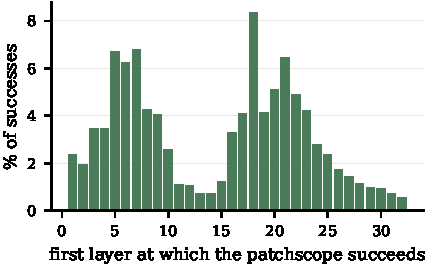
\includegraphics[width=\columnwidth]{figures/first_successful_layer}
\caption{Over the full $32$-layer sweep with context, the first layer at which
the patchscope recovers the target, as a fraction of all successes.}
\label{fig:firstlayer}
\end{figure}

Figure~\ref{fig:firstlayer} shows, across the $26{,}015$ successful in-context
trials of the $32$-layer sweep, which layer first produced the target. The
distribution has two modes, one around L5--L8 and a larger one around L18--L22;
the median is L16 and $41.9\%$ of successes first appear at or before L10. The
early mode is not visible in the eight-layer analysis of \S\ref{sec:layers},
which samples only L5 and L7 below L10.

\subsection{Probe generalisation to unseen categories}

Training the generation-label probe on two phrase categories and testing on the
third costs accuracy but does not eliminate the signal. Against a no-hold-out
baseline of $73.6\%$ / $74.6\%$ / $76.8\%$ balanced accuracy at L13 / L25 / L30,
holding out landmarks gives $69.1\%$ / $62.6\%$ / $63.4\%$, idioms
$68.7\%$ / $68.9\%$ / $72.3\%$, and film titles
$72.4\%$ / $72.7\%$ / $73.5\%$. Landmarks are the hardest category to
generalise to, which is unsurprising given that they are only $5.7\%$ of pooled
instances. The probe is therefore learning something that partly transfers
across phrase types rather than memorising category-specific surface features,
but the transfer is imperfect --- a pattern also reported by
\citet{orgad-etal-2025-llms} for truthfulness probes across datasets.

\subsection{Per-phrase correlation between probe confidence and difficulty}

A complementary check on whether the probe tracks phrase identity: for each test
phrase, we compare the probe's mean predicted probability across that phrase's
contexts with the phrase's true success rate. At $i=3$ over $180$ test phrases,
Pearson correlation by layer is $0.413$ (L5), $0.551$ (L7), $0.621$ (L10),
$0.584$ (L13), $0.603$ (L15), $0.556$ (L20), $0.517$ (L25) and $0.480$ (L30) ---
a broad mid-network peak. The probe's confidence therefore varies with which
phrase it is looking at, not only with generic features of the position.

\subsection{Reproducing the numbers}

Every number in the main text except Table~\ref{tab:probes} and the
adjudication of \S\ref{sec:falsepos} is recomputed from the files in
\texttt{results/raw/} by \texttt{code/make\_paper\_numbers.py}, which writes
\texttt{results/processed/paper\_numbers.json}; the tables and figures are
generated from that file by \texttt{code/make\_tables.py} and
\texttt{code/make\_figures.py}. The experiment scripts are in
\texttt{code/phrase\_recognition/}. Per-trial hidden states, which the probing
experiments require, are not distributed.
